\section{GUI modelling}

From the application specifications, I built the \textit{flowchart} (schematic representation of a sequence of actions) of user interaction on the different pages of the application, see appendix \ref{appendix:ihm}. First of all, I listed the different pages that the application must be composed. A page is represented by a rectangle with the name of the page with by a brief description. Navigation between two pages is represented by a directional arrow to the destination page with the trigger that causes the page to change (represented by a diamond).

\begin{figure}[H]
  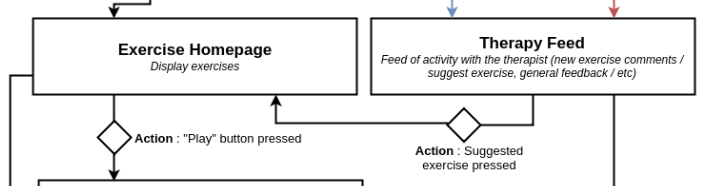
\includegraphics[width=.8\linewidth]{content/imgs/ihm_ex.png}
  \caption{Example of flowchart between pages \textit{Exercice Homepage} and \textit{Therapy Feed}}
  \label{fig:flowchart}
\end{figure}

From the application specifications, I built the \textit{flowchart} (schematic representation of a sequence of actions) of user interaction on the different pages of the application, see appendix \ref{appendix:ihm}. A \textit{wireframe} is a functional mock-up, i.e. a schematic representation of the interface in order to define the different components of the interface without worrying about its design rules -- such as colors or typography for example. The \textit{wireframes} focus on the ergonomics of the application and not on the design of the application. The \textit{wireframe} of a stuttering user's main page is available in the figure \ref{fig:wireframe} .


\begin{figure}[H]
  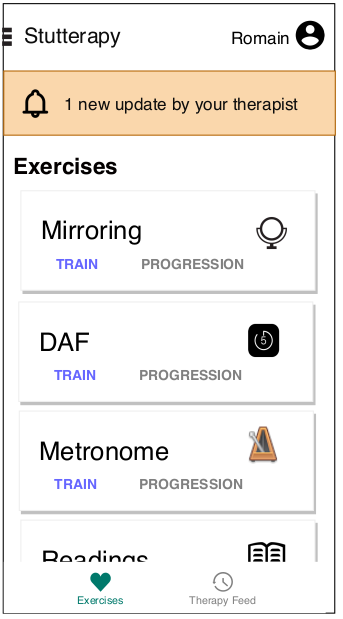
\includegraphics[width=.3\linewidth]{content/imgs/wireframe_ex.png}
  \caption{\textit{Wireframe} of stutterer main page}
  \label{fig:wireframe}
\end{figure}
